\subsubsection{Schrittmotor}
Der Schrittmotor dient der horizontalen Ausrichtung des Maschinenturms.
Hierzu ist der Schrittmotor fix eingebaut im Turm und greift per Zahnrad
in einen Kranz der Bodenplatte. Mit dem Drehen des Zahnrades rotiert der
Turm zur entsprechenen Seite. Hierfür ist ein Schrittmotor vom Typ 
QSH4218-51-10-049 von Trinamic.

\begin{figure}[h!]
	\centering
	\begin{subfigure}[b]{0.45\textwidth}
		\centering
		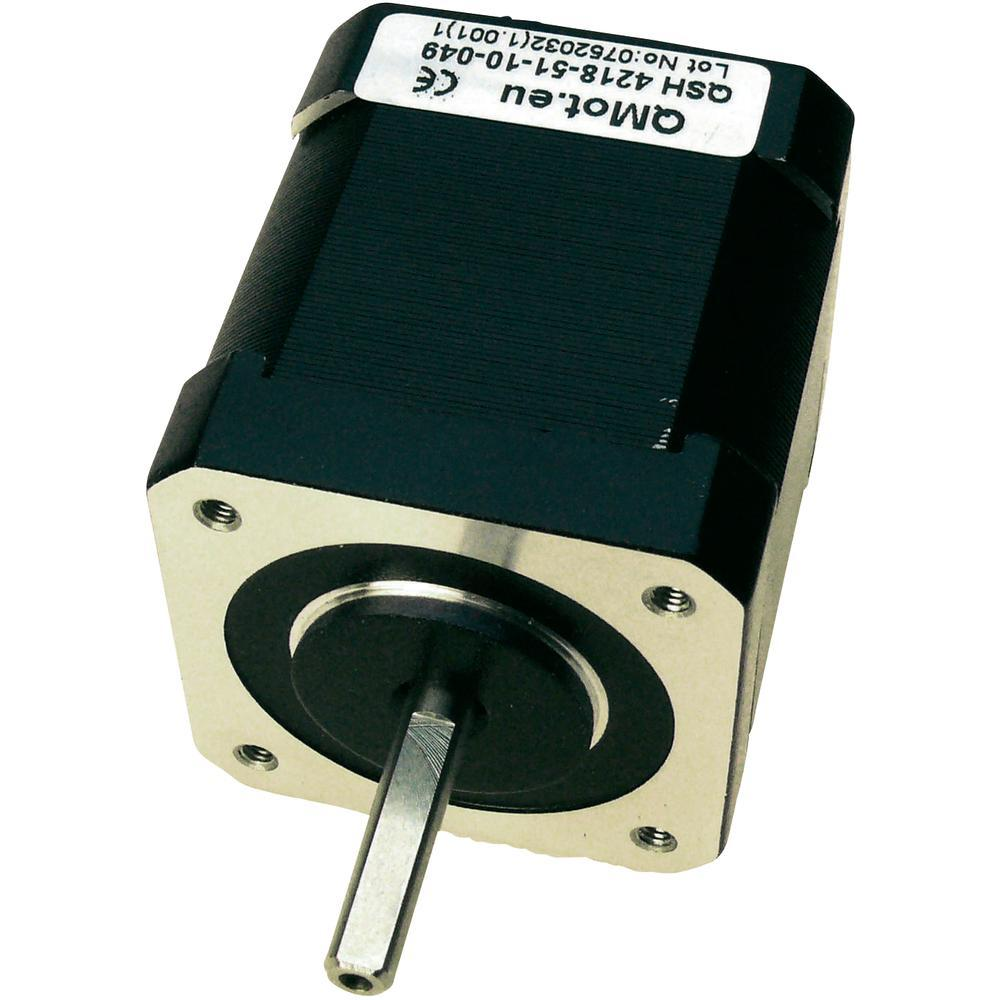
\includegraphics[width=1\textwidth]{../../fig/et/QSH4218-51-10-049.jpg}
		\caption{Schrittmotor QSH4218-51-10-049}
	\end{subfigure}
	\begin{subfigure}[b]{0.45\textwidth}
		\centering
		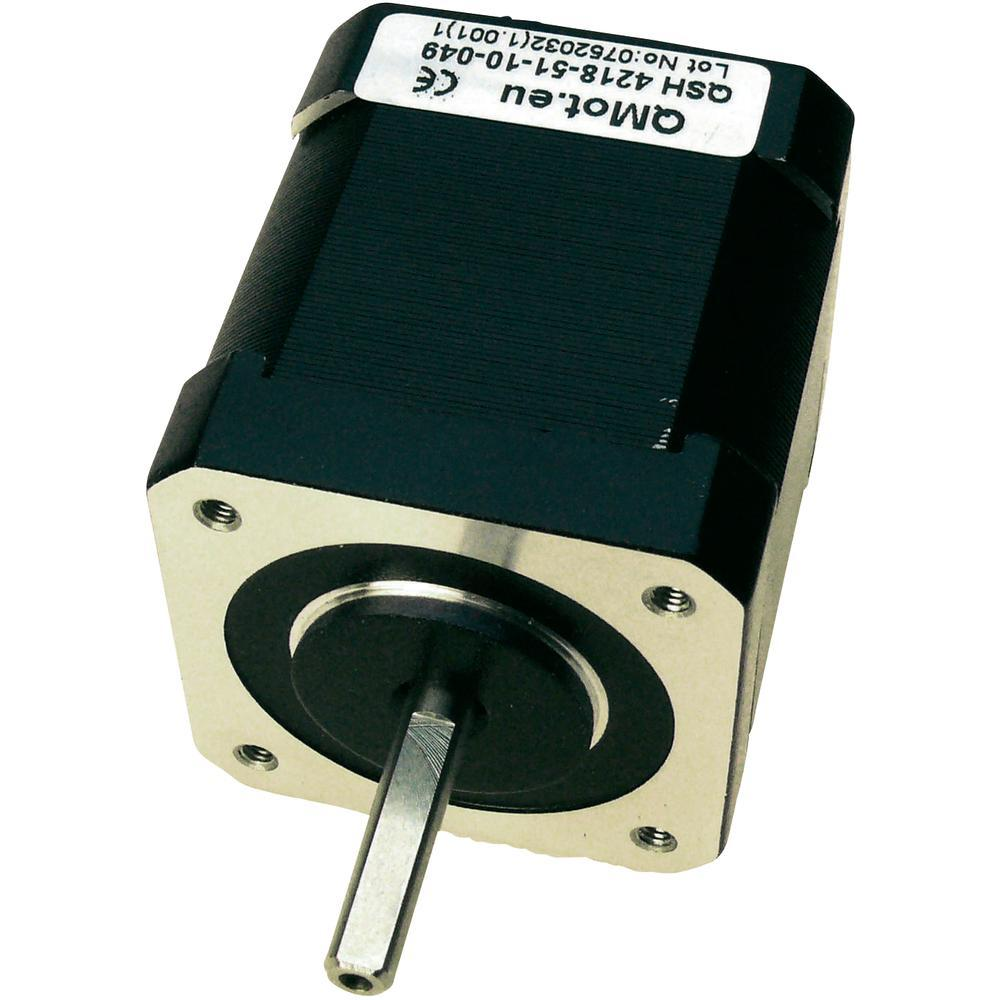
\includegraphics[width=1\textwidth]{../../fig/et/QSH4218-51-10-049.jpg}
		\caption{Stepper-Treiberboard von PREN-ET}
	\end{subfigure}
	\caption{Motor und Elektronik des Schrittmotors}
\end{figure}

Für die Ansteuerung des Schrittmotors ist ein von der Gruppe PREN-ET
entwickeltes Shield für das Freedomboard im Einsatz. Dieses beinhaltet
als Kernkomponente den Treiberchip L6480 von ST Microelectronics. Dieser
implementiert sämtliche Funktionalitäten und Ansteuerungsverfahren für den
Schrittmotor inklusive Optimierungsmöglichkeiten. Der Chip wird dabei
mittels einer SPI Verbindung von Freedomboard aus gesteuert.
